\documentclass[12pt,a4paper]{article}
\usepackage[utf8]{inputenc}
\usepackage[T1]{fontenc}
\usepackage{graphicx}
\usepackage{tikz}
\usetikzlibrary{positioning}
\usepackage{xcolor}
\usepackage{geometry}
\usepackage{hyperref}
\usepackage{enumitem}
\usepackage{booktabs}

\geometry{margin=1in}

\title{\textbf{Section X: Cybersecurity \& Cyber-Resilience Strategy for Sovereign Cloud/Edge Computing}}
\author{}
\date{}

\begin{document}

\maketitle

\tableofcontents
\newpage

\begin{figure}[h!]
        \centering
        \resizebox{\textwidth}{!}{%
        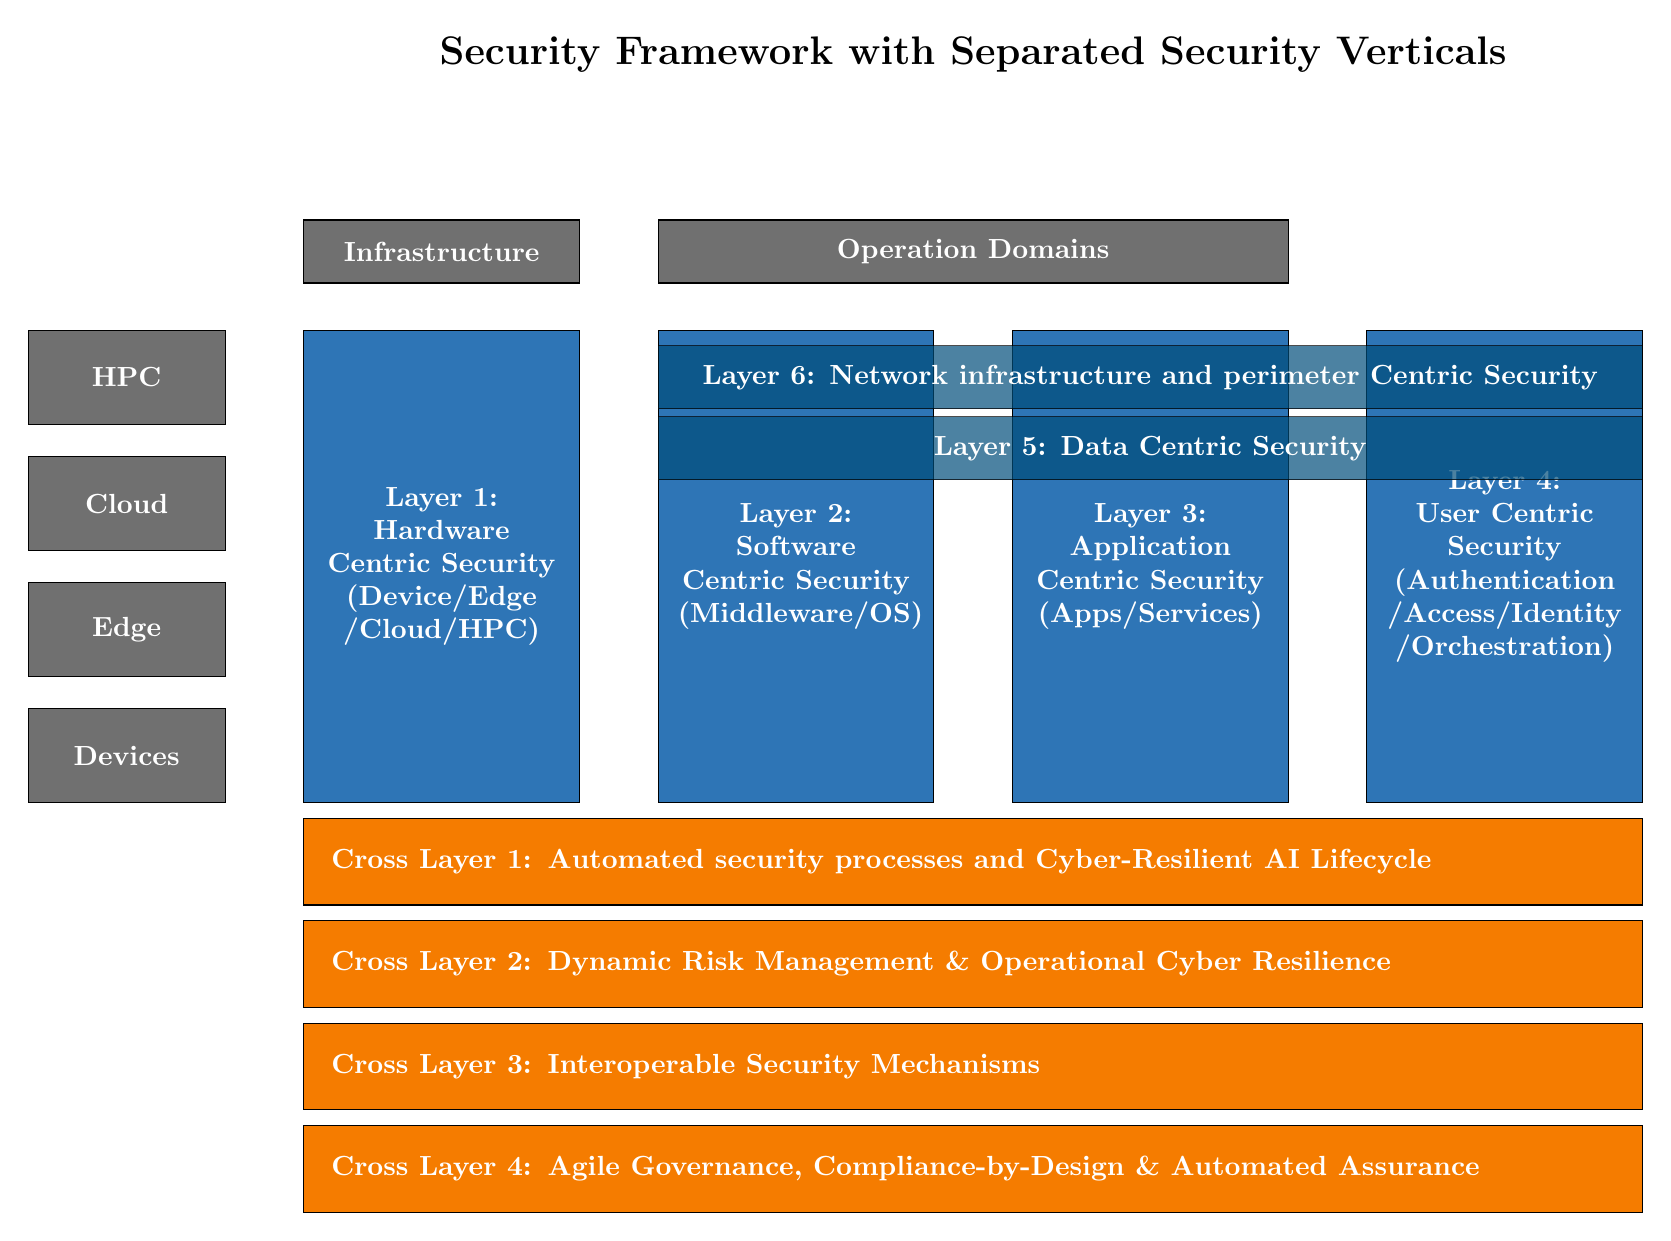
\begin{tikzpicture}[every node/.style={font=\small}]
            % Define colors
            \definecolor{archblue}{RGB}{46, 117, 182}
            \definecolor{sec_verticals_bg}{RGB}{245, 124, 0}
            \definecolor{env_bg}{RGB}{112, 112, 112}
            \definecolor{overlay}{RGB}{0, 77, 122}

            % Styles
            \tikzstyle{arch_col} = [fill=archblue, draw=black, text=white, font=\bfseries, minimum width=3.5cm, minimum height=6cm, align=center, text width=3cm]
            \tikzstyle{env_box} = [fill=env_bg, draw=black, text=white, font=\bfseries, minimum width=2.5cm, minimum height=1.2cm, align=center]
            \tikzstyle{top_tool} = [draw=black, fill=env_bg, text=white, minimum height=0.8cm, align=center, font=\bfseries]
            \tikzstyle{overlay_box} = [fill=overlay, draw=black, text=white, font=\bfseries, minimum height=0.8cm, align=center, opacity=0.7, text opacity=1]
            \tikzstyle{vertical_box} = [fill=sec_verticals_bg, draw=black, text=white, font=\bfseries, minimum width=17.0cm, minimum height=1.1cm, align=left, text width=16.3cm]

            % Column X positions
            \def\colone{-4.5}
            \def\coltwo{0}
            \def\colthree{4.5}
            \def\colfour{9}

            % Environment boxes (left)
            \node[env_box] at (-8.5, 2.4) {HPC};
            \node[env_box] at (-8.5, 0.8) {Cloud};
            \node[env_box] at (-8.5, -0.8) {Edge};
            \node[env_box] at (-8.5, -2.4) {Devices};

            % Main architecture columns representing layers
            \node[arch_col] (hw) at (\colone, 0) {Layer 1: \\ Hardware Centric Security \\ (Device/Edge\\ /Cloud/HPC)};
            \node[arch_col] (mw) at (\coltwo, 0) {Layer 2: \\ Software Centric Security \\ (Middleware/OS)};
            \node[arch_col] (app) at (\colthree, 0) {Layer 3: \\ Application Centric Security \\ (Apps/Services)};
            \node[arch_col] (user) at (\colfour, 0) {Layer 4: \\ User Centric Security \\ (Authentication\\ /Access/Identity\\ /Orchestration)};

            % Top tooling boxes
            \node[top_tool, minimum width=3.5cm] at (\colone, 4) {Infrastructure};
            \node[top_tool, minimum width=8cm] at (2.25, 4) {Operation Domains};

            % Arrows from tooling
            \draw[->, line width=2pt, white] (\colone, 3.5) -- (\colone, 3.1);
            \draw[->, line width=2pt, white] (2.25, 3.5) -- (2.25, 3.1);

            % Other layers as overlays/headers
            \node[overlay_box, minimum width=12.5cm] at (4.5, 1.5) {Layer 5: Data Centric Security};
            \node[overlay_box, minimum width=12.5cm] at (4.5, 2.4) {Layer 6: Network infrastructure and perimeter Centric Security};

            % Separated vertical boxes
            \node[vertical_box] at (2.25, -3.75) {\textbf{Cross Layer 1: Automated security processes and Cyber-Resilient AI Lifecycle}};
            \node[vertical_box] at (2.25, -5.05) {\textbf{Cross Layer 2: Dynamic Risk Management \& Operational Cyber Resilience}};
            \node[vertical_box] at (2.25, -6.35) {\textbf{Cross Layer 3: Interoperable Security Mechanisms}};
            \node[vertical_box] at (2.25, -7.65) {\textbf{Cross Layer 4: Agile Governance, Compliance-by-Design \& Automated Assurance}};

            % Title
            \node[font=\Large\bfseries, anchor=center] at (2.25, 6.5) {Security Framework with Separated Security Verticals};

        \end{tikzpicture}%
        }
        \caption{Security Framework with separated security verticals in dedicated boxes.}
        \label{fig:security_framework_verticals_boxes}
    \end{figure}

\noindent\textbf{Topic:} Cybersecurity for the Cognitive Computing Continuum\\
\textbf{Destinations:}
\begin{itemize}
    \item \textbf{Primary:} 4. A secure, sovereign European computing continuum infrastructure.
    \item \textbf{Secondary:} 6. European leadership in emerging disruptive computing paradigms.
\end{itemize}

\section{Background \& Driving Factors}
\begin{itemize}
    \item \textbf{Decentralization Risk:} The paradigm shift from the centralized Cloud to a distributed Cloud-Edge-IoT continuum radically expands the attack surface. Traditional perimeter-centric models cannot cope with this dispersion.
    \item \textbf{Physical Exposure:} Edge nodes and far-edge IoT devices frequently operate in unprotected field environments where tampering, side-channel attacks, and physical extraction are viable attack vectors.
    \item \textbf{Regulatory Pressure:} EU rollout of NIS2 \cite{nis2}, CRA \cite{cra}, and the AI Act \cite{aiact} requires consistent compliance across a fragmented landscape that lacks baseline interoperability.
    \item \textbf{Digital Sovereignty:} Dependence on non-EU cloud providers and trust anchors exposes EU data and AI pipelines to extraterritorial access and geopolitical risk.
\end{itemize}

\section{Europe in Relation to the State of the Art}
\textbf{Comparison vs. Hyperscalers:}
\begin{itemize}
    \item \textbf{EU Strengths:} Europe leads globally in trust, privacy engineering, and the deployment of rigorous certification schemes (e.g., EUCS \cite{eucs}). 
    \item \textbf{EU Gaps:} The market trails hyperscalers in unified security orchestration and lacks sovereign silicon capacity, showing fragmentation in threat-intelligence sharing.
\end{itemize}
\textbf{Strategic Goal:} Transition the EU from reactive, siloed cybersecurity to autonomous, federated, and certified Security-by-Design across the computing continuum.

\section{Strategic Preamble}
This section defines the architectural guardrails that secure the Cloud-Edge-IoT Continuum, replacing legacy perimeter defenses with distributed cyber-resilience. 
\begin{itemize}
    \item \textbf{Capability Profiles (Qualitative):} Deep 7-dimensional analysis defining what must be built to ensure sovereignty.
    \item \textbf{Progression Matrix (Quantitative):} Evolution tracked via Operational Deployment Phases (ODP) and Strategic Sovereignty Levels (SSL).
\end{itemize}

\section{The Core Capability Dimensions (Architectural Framework)}
The roadmap is structured across a cohesive architectural framework that spans four continuum environments (HPC, Cloud, Edge, Devices).

\subsection*{Part A: The Security Layers (Vertical Stack)}
\begin{description}
\item[Layer 1.1 Hardware Roots of Trust:] Cryptographically verifiable supply chain trust ensuring physical device integrity. Drive European open-hardware (e.g., RISC-V) toward \textbf{EUCC 'High' assurance} certification \cite{eucc} to guarantee resistance against tampering at the vulnerable far-edge.

\item[Layer 2.1 OS \& Middleware Hardening:] Securing hypervisors and distributed operating systems. This involves hardening KVM/QEMU and supporting sovereign Linux distributions optimized for edge resource constraints.

\item[Layer 3.1 Workload Security:] Securing containerized applications and serverless functions executing dynamically. Implementation of hardened service meshes provides mutual TLS and granular traffic inspection without performance degradation.

\item[Layer 4.1 Zero-Trust Orchestration:] Seamless policy enforcement across providers requiring robust PEP/PDP architectures. This enables continuous authorization and dynamic access controls that adapt to the context of the request.

\item[Layer 4.2 Federated Identity (IAM):] Cross-domain identity federation using Self-Sovereign Identity (SSI) principles. This allows for cryptographically secure, decentralized authentication for machines, users, and workloads.

\item[Layer 5.1 End-to-end Confidential Computing:] Data-in-use security through Trusted Execution Environments (TEEs). Leveraging TEE abstraction layers ensures sensitive European data remains encrypted during processing.

\item[Layer 5.2 Post-Quantum \& Cryptographic Agility:] PQC standardization and hybrid crypto deployment to secure long-lived data against "Harvest Now, Decrypt Later" quantum threats.

\item[Layer 6.1 Telco-cloud \& O-RAN Security:] Hardening distributed 5G/6G cores in strict alignment with the \textbf{SNS JU SRIA} \cite{snsju}. This ensures sovereign control over network slice isolation.

\item[Layer 6.2 Physical Resilience \& Safety:] Adapting strict network controls and IT/OT gateway security for high-availability edge environments (e.g., Smart Grids) to prevent digital breaches from causing kinetic damage.
\end{description}

\subsection*{Part B: The Transversal Security Verticals (Cross-Layers)}
\begin{description}
\item[CL1.1 Continuous DevSecOps (Shift-Left):] Embedding AI-driven code analysis and automated vulnerability remediation at the earliest stages of the software lifecycle.

\item[CL2.1 Automated SOC Operations:] Continuous monitoring and SOC federation across Member States using legally protected, cross-border threat intelligence platforms \cite{concordia}.

\item[CL3.1 Interoperability \& Simpl Integration:] Secure communication across disparate systems via mandatory integration into the \textbf{Simpl} smart middleware \cite{cloud_edge_roadmap} to unlock \textbf{Common European Data Spaces}.

\item[CL4.2 Continuous Automated Certification:] Replacing point-in-time audits with real-time certification tracking for both cloud services (\textbf{EUCS}) and physical edge products (\textbf{EUCC}) \cite{eucc}.
\end{description}

\section{The 4-Filter Prioritization Framework}
To ensure the roadmap provides actionable guidance, capabilities are prioritized using a structured 4-filter logic:
\begin{enumerate}
    \item \textbf{Regulatory Urgency:} Capabilities required to comply with imminent law (NIS2, CRA, AI Act).
    \item \textbf{Foundational Dependency:} Technologies (e.g., Layer 1 Hardware Trust) that must exist for other layers to function.
    \item \textbf{The Sovereignty Cliff:} Prioritizing areas where the EU has 100\% foreign dependency or faces immediate "extinction" threats (e.g., Q-Day).
    \item \textbf{Market Feasibility:} Alignment with existing investments like \textbf{Simpl} and adoptability by SMEs.
\end{enumerate}

\section*{Executive Priorities: The Critical Path (Phase 1)}
Applying the 4-Filter Framework, the immediate strategic priorities are:
\begin{itemize}
    \item \textbf{Priority 1:} Hardware Roots of Trust \& EUCC 'High' Certification.
    \item \textbf{Priority 2:} Post-Quantum Cryptographic Agility for Edge/IoT.
    \item \textbf{Priority 3:} Security Interoperability via Simpl Middleware.
\end{itemize}

\section{Capability Profiles \& Progression Matrices}

\subsection*{Priority 1: Hardware Roots of Trust \& EUCC 'High'}
\begin{enumerate}
\item \textbf{Baseline \& Target Objective:} Current baseline relies on foreign proprietary TPMs. Target is ubiquitous deployment of EU-designed, open-source (RISC-V) enclaves with \textbf{EUCC 'High'} certification.
\item \textbf{Primary Drivers:} Regulatory mandates under \textbf{CRA} and the threat of state-level physical tampering on decentralized edge nodes.
\item \textbf{High Impact Activities:} Development of sovereign Secure Elements based on RISC-V and automated hardware-level remote attestation.
\item \textbf{Catalysts \& Enablers:} \textbf{EU Chips Act} pilot lines and \textbf{ECCC Strategic Agenda} funding alignment.
\item \textbf{Disruptors:} Supply chain bottlenecks and breakthroughs in physical side-channel analysis.
\item \textbf{Failsafe Mechanisms:} node isolation protocols and software-based TEE redundancy.
\item \textbf{Transversal Meta-Layer:} Eliminates "black-box" dependencies and promotes energy-efficient (Green IT) secure silicon.
\end{enumerate}

\vspace{0.5cm}
\noindent\textbf{Progression Matrix: Hardware Roots of Trust}
\vspace{0.2cm}

\noindent
\resizebox{\textwidth}{!}{%
\begin{tabular}{@{}llll@{}}
\toprule
\textbf{Metric} & \textbf{Phase 1 (0-5 Yrs)} & \textbf{Phase 2 (5-10 Yrs)} & \textbf{Phase 3 (10-15 Yrs)} \\ \midrule
\textbf{ODP} & Fragmented Piloting & Standardized Integration & Ubiquitous Operation \\
\textbf{SSL} & High Foreign Dependency & Emerging EU Ecosystem & Full Sovereign Autonomy \\
\textbf{State} & RISC-V pilots begin. & EU elements in critical infra. & Sovereign trust by default. \\
\textbf{Enabler} & \textbf{CRA} Enforcement & \textbf{EUCC 'High'} Certification & \textbf{EU Chips Act} Maturity \\ \bottomrule
\end{tabular}%
}

\begin{thebibliography}{99}
\bibitem{nis2} European Parliament and Council, ``NIS2 Directive,'' Dec. 2022.
\bibitem{cra} European Commission, ``Cyber Resilience Act,'' Sep. 2022.
\bibitem{aiact} European Parliament and Council, ``AI Act,'' Jun. 2024.
\bibitem{eucs} ENISA, ``EUCS Scheme,'' Dec. 2020.
\bibitem{eucc} ENISA, ``EUCC Scheme,'' Jul. 2020.
\bibitem{cloud_edge_roadmap} European Alliance for Industrial Data, ``Cloud-Edge Roadmap,'' 2024.
\bibitem{snsju} SNS JU, ``SRIA Agenda,'' 2023.
\bibitem{concordia} G. Dreo et al., ``CONCORDIA Roadmap,'' Dec. 2022.
\end{thebibliography}

\end{document}